\section{Diffusion Transformer (DiT)}
\label{appendix:diffusion_transformer}

\begin{figure}
    \centering
    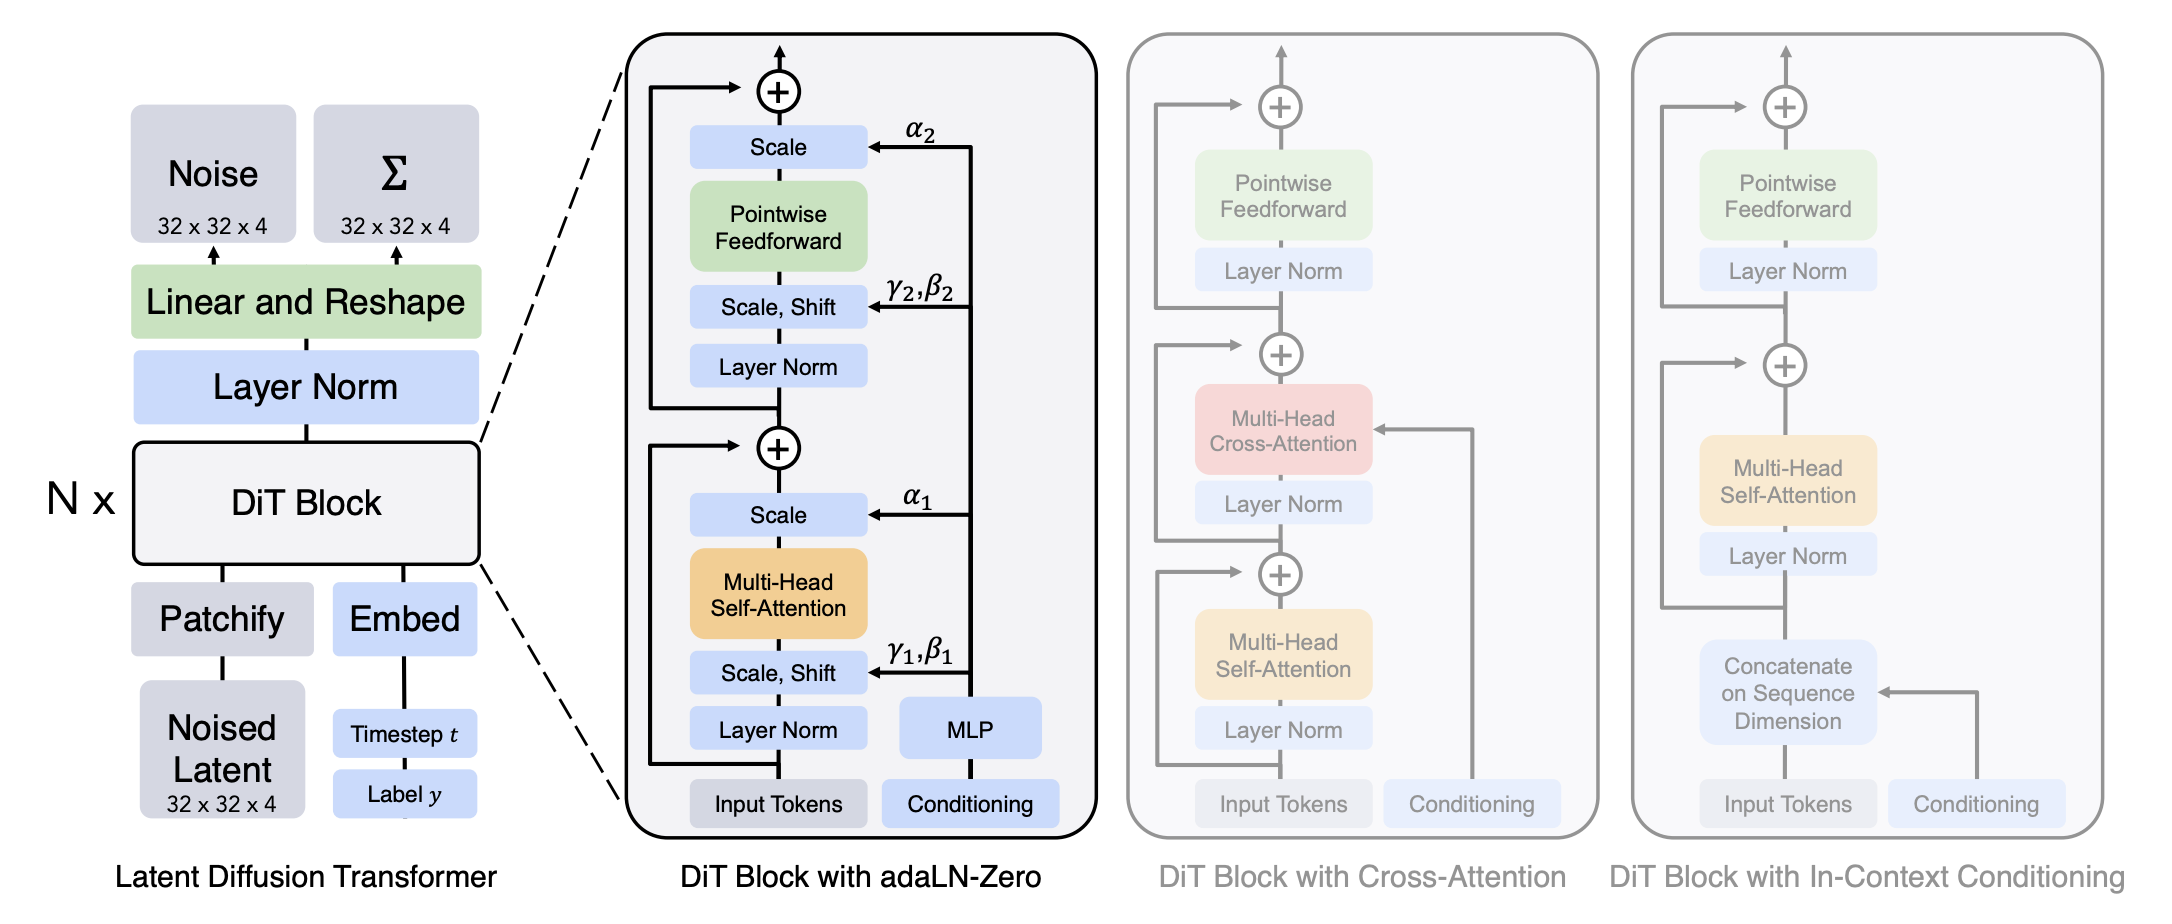
\includegraphics[width=0.8\textwidth]{images/appendix/diffusion_transformer/architecture.png}
    \caption{Diffusion Transformer (DiT) architecture \cite{diffusion_transformer}. \textit{Right}: three DiT blocks: with adaLN (adaptive layer normalization), cross-attention, and in-context conditioning \cite{diffusion_transformer}.}
    \label{fig:diffusion_transformer_architecture}
\end{figure}


Diffusion Transformer (DiT), introduced in 2023 \cite{diffusion_transformer}, is a diffusion model based on transformers. It replaces the U-Net in LDMs with a transformer for latent denoising. Leveraging transformers' scalability capabilities, DiT reduces computational complexity (measured in Gflops) and improves sample quality, achieving a state-of-the-art FID score of 2.27 on ImageNet.

Inspired by Vision Transformer (ViT) \cite{vision_transformer}, DiT processes images by dividing them into patches, embedding each as tokens with added positional encodings, and feeding these into the transformer blocks.

\textbf{In-context conditioning block}: Class labels and diffusion time embeddings are added as conditioning tokens to the input sequence, similar to the \texttt{[CLS]} token in ViT (added at the beginning of the input sequence). They are removed after processing, and the transformer decoder can perform the noise prediction task.

\textbf{Cross-attention block}: In similar manner to LDMs, they use cross-attention with the class label $c$ and diffusion timestep embeddings $t$ and feed it into cross-attention, where the other input sequence (sequence of patch + position embeddings) is used as the query.

\textbf{Noise prediction \& diagonal covariance matrix}: The output of the model is learned noise prediction and a diagonal covariance matrix $\sum_\theta$ (shown in figure \ref{fig:diffusion_transformer_architecture}). We optimize $\sum_\theta$ in order to optimize the decoder $\mathcal{D}_{KL}$.

